% \section{$k$-clique}

$k$-clique problem belongs to NP-complete problems. Note that $k$-clique problem in $G$ is equivalent to $n-k$ independent set in $\overline{G}$ so we can assume $k \leq \frac{n}{2}$. Like before we add an unchecked vertex if $k$ is odd so we will assume $k$ to be even. % možná: and there exists a DNA system with very low complexity: $\min\bigl\{ 1\nicefrac{1}{4}\;\bigl( \frac{n}{2} \bigr) ^2 ,\; 1\nicefrac{1}{4}\;k^2 \bigr\}$.

\subsection*{Set of tiles}

\begin{description}
	\item[Bottom line] For now there are tiles with $2l-2$ and $2l$ ($0 < l \leq \frac{k}{2}$) on the bottom and with an arbitraty ordered\footnote{Note that this restriction does not reduce the set of possible $k$-member subsets.} pair of different numbers from $1$ to $n$ with $k-2l+2$-th and $k-2l+1$-th colors, respectively, on the top. Note that now the order of colors is given and do not forget that they should also contain those upper sequences once more on the bottom strand. $\frac{kn^2}{4}$ tile types were required. % na prvních místech nejnižší čísla, na nejvyšších ty nejvyšší -> sníží počet dlaždic ale je s tim sraního
	\item[Bottom corner tiles] Are exactly the same. $2$ tile types were required.
	\item[Inner tiles] These tiles are now responsible for ordering by color during which they check existence of {\em every} edge in similar manner to previous problems. And because the first line contains them in reverse order there will meet each other. $k^2 n^2$ tile types were required. % $k^2 \cdot 2#E $
	\item[Border tiles] These tiles are exactly the same like for 3-coloring.
	\item[Checking tiles] As soon as the most left color reaches sharp and the most right color reaches asterisk, checking is triggered in similar manner to 3-coloring. $kn$ tile types were required.
	\item[DONE tile] This is exactly the same like 3-coloring. $1$ tile type was required.
\end{description}
Summed up, this DNA algorithm requires $k^2 n^2$ tile types. % $k^2 \cdot 2#E $

\begin{figure}[H]
\begin{center}
	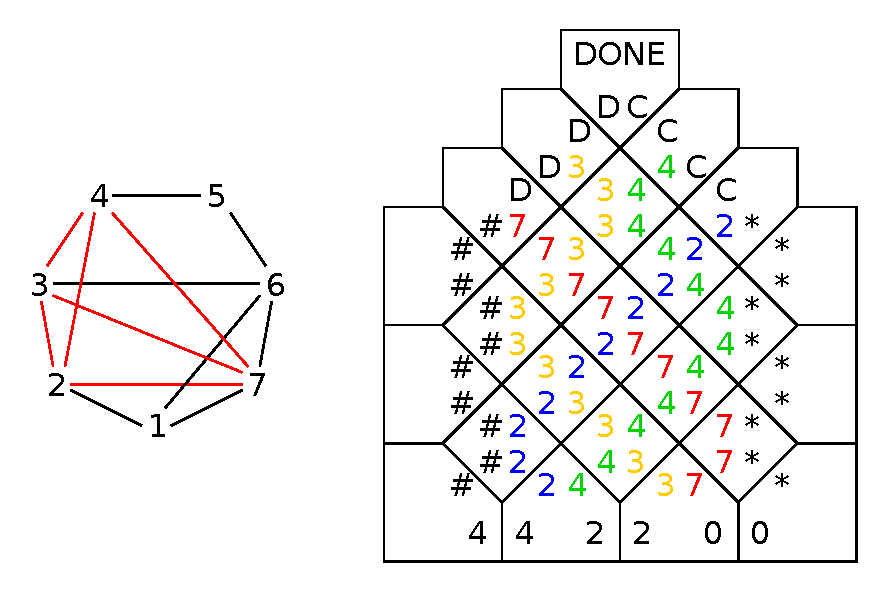
\includegraphics[scale=0.75]{./figures/k-clique/k-clique.pdf}
	\caption{$k$-clique computation. Color order is defined by their wavelength.}
	\label{fig:graph_iso}
\end{center}
\end{figure}

